\chapter{Datasets description}


Con el fin del modelado del sistema completo del invernadero describiremos las bases de datos disponibles de este. Como veremos tenemos una gran cantidad de información en las variables de clima, mientras que las medidas  crecimiento de la plantación se reduce a la producción del fruto. Además procederemos a explicar un preprocesado preliminar que podemos realizar sin necesidad de tener en cuenta los modelos de clima, ni de crecimientos. Este constará de un eliminación de ruido y una pre-selección de variables con información relevante

En este capítulo seguiremos de la siguiente manera: (1) Presentaremos las bases de datos históricos en bruto tal y como se recogieron antes de empezar el proyecto, realizando pequeñas modificaciones. (2) Realizaremos un análisis de correlaciones lineales preliminar con el fin de remover variables linealmente dependientes. 
\section{Datos Disponibles}


El invernadero consta de un sistema de captura de datos llamado \emph{sysclima}, enfocado en las variables climáticas, a continuación la describiremos la base de datos capturado por \emph{sysclima}. 

\subsection{Datos Brutos}
\begin{dataset}[SysClima Bruto]\label{dataset:sysclima}
    Serie temporal de variables climáticas con una frecuencia de muestreo no uniforme de aproximadamente $2$ minutos. Además de las variables de clima esta base de datos contiene información sobre el estado de la pantalla de sombreo y del porcentaje de apertura de las ventanas, variables que podemos considerar como variables manipulables. Mostramos una descripción detallada de las variables en la tabla \ref{table:SysClimaDS} y una representación gráfica en la Figura \ref{fig:ViewDataSetSysClima}.
\end{dataset}

\begin{table}
    \centering
    \begin{tabular}{|c|c|c|c|}
        \hline
        \textbf{Name}           & \textbf{Units} & \textbf{Description}         \\ 
        \hline
        \texttt{Time Stamp}         & -              &                              \\ \hline
        \texttt{Var2}               & -              & Sección de invernadero       \\ \hline
        \texttt{Text}               & $^\circ C$     & Temperatura exterior         \\ \hline
        \texttt{HRExt}              & \%             & Humedad relativa Exterior    \\ \hline
        \texttt{RadExt}             & $W/m^2$        & Radiación Exterior           \\ \hline
        \texttt{Vviento}            & $km/s$         & Wind Velocity                \\  \hline
        \texttt{DireccinViento}     & $^\circ$       & Dirección del Viento         \\ \hline
        \texttt{RadAcumExt}         & $W/m^2$        & Radiación Acumulada diaria Exterior \\ \hline
        \texttt{AlarmaLluvia}       & -              & Alarma de Viento             \\ \hline
        \texttt{AlarmaVto}          & -              & Alarma de Lluvia             \\ \hline
        \texttt{Tinv}               & $^\circ C$     & Temperatura interior         \\ \hline
        \texttt{Troco}              & $^\circ C$     & Temperatura de Rocio         \\  \hline
        \texttt{RadInt}             & $W/m^2$        & Radiación Interior               \\ \hline
        \texttt{xDemPant1}          & $\%$           & Demanda de Pantalla de Sombreo   \\ \hline
        \texttt{xEstadoPant1}       & $\%$           & Estado de Pantalla de Sombreo    \\ \hline
        \texttt{TVentilacin}        & $^\circ C$     & Temperatura de Ventilación       \\ \hline
        \texttt{EstadoCenitalE}     & $\%$           & Porcentaje de apertura Cenital Este      \\ \hline
        \texttt{EstadoCenitalO}     & $\%$           & Porcentaje de apertura Cenital Oeste     \\ \hline
        \texttt{MaxHR}              & $\%$           & Maxima Humedad Relativa      \\ \hline
        \texttt{MinHR}              & $\%$           & Mínima Humedad Relativa      \\ \hline
        \texttt{DeltaX}             & $g/m^3$        &                              \\ \hline
        \texttt{DeltaT}             & $^\circ C$     &                              \\ \hline
        \texttt{DPV}                & $mbar$         & Déficit de Presión de Vapor  \\  \hline
        \texttt{HRInt}              & $\%$           & Humedad relativa Interior    \\ \hline
        \texttt{Ventiladores2Activo}&    -            &         -                    \\ \hline
        \texttt{Aerotermo1Activo}   &    -           &         none                    \\ \hline
        \texttt{Sonda1}             &                &        none                    \\ \hline
        \texttt{Sonda2}             &                &         -                    \\ \hline
        \texttt{Sonda3}             &                &         -                    \\ \hline
        \texttt{Sonda5}             &                &         -                    \\ \hline
        \texttt{Sonda6}             &                &         -                    \\
        \hline
    \end{tabular}
    \caption{Variables of dataset \ref{dataset:sysclima}}
    \label{table:SysClimaDS}
\end{table}

\begin{figure}[ht!]
    \centering
    \includegraphics[scale=0.65]{img/SysClimaDataSet.eps}
    \caption{Preliminary view of Dataset \ref{dataset:sysclima} from Jul-2016 to Jun-2019 }
    \label{fig:ViewDataSetSysClima}
\end{figure}

Por razones que profundizaremos más adelante ha sido necesario obtener datos climáticos de la estación meteorológica de Derio. Este es la estación más cercana al invernadero de Meñaka con históricos que coinciden temporalmente con los datos del DataSet \ref{dataset:sysclima}

\begin{dataset}[Meteorologic Station of Derio - Euskalmet]\label{dataset:Euskalmet}
    Serie temporal de variables climática de la estación meteorológica de Derio, desde 2016 hasta 2020 con una frecuencia de muestro de diez minutos. Utilizaremos esta base de datos de clima con el fin de complementar las regiones sin medidas de la base de datos \ref{dataset:sysclima}.
\end{dataset}

Por otro lado, como hemos mencionado anteriormente el único registro claro con respecto al crecimiento de la plantación la masa de fruto recogido. Este registro se encuentra en la siguiente base de datos.

\begin{dataset}[Tomatoes Production]\label{dataset:ProductionMenaka}
    Serie temporal de masa de tomates producidos con una frecuencia de muestreo aproximada diaria y medido en kilogramos. Estos datos son recogidos manualmente por el personal del invernadero.
\end{dataset}

\begin{figure}
    \centering
    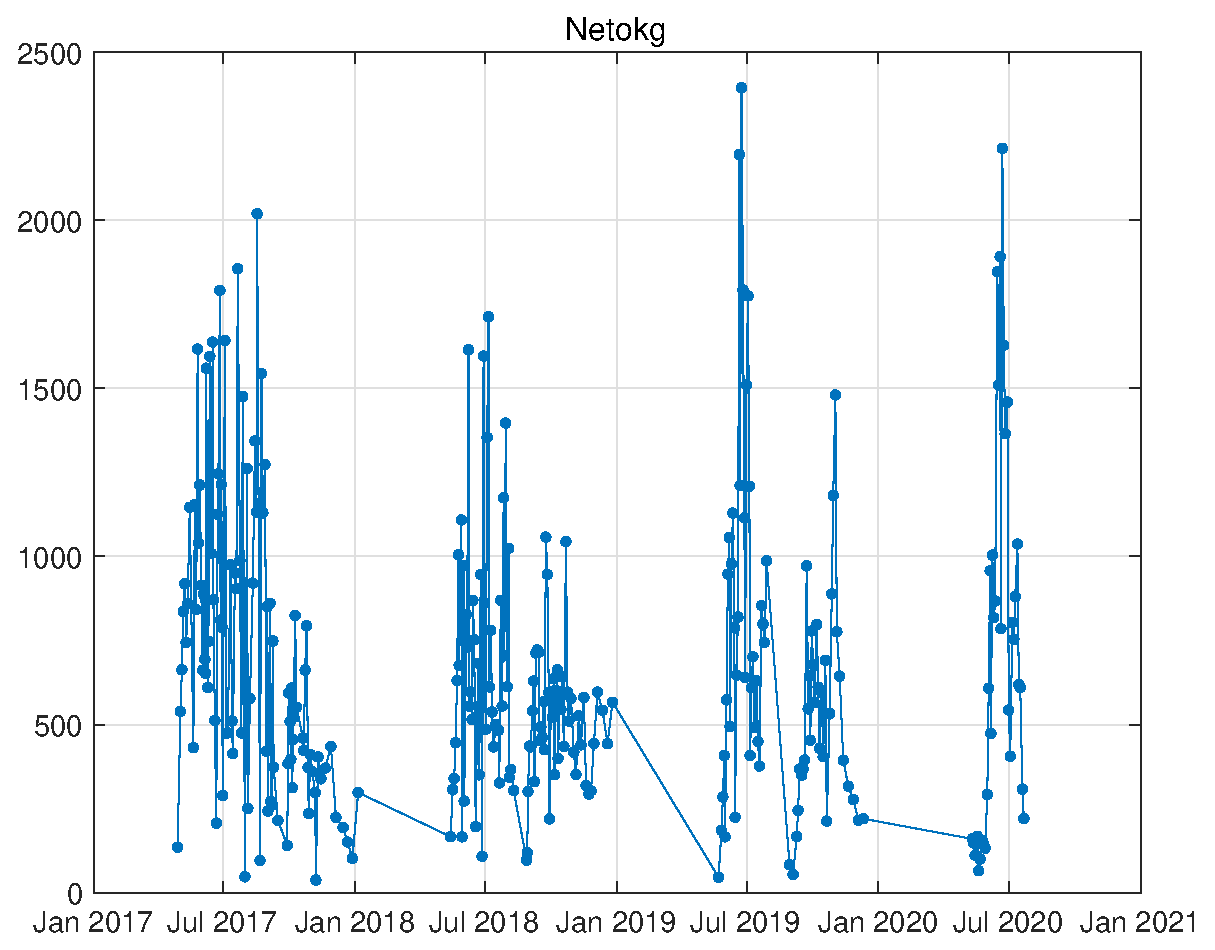
\includegraphics[scale=0.4]{img/ProdMenaka.eps}
    \caption{View of Dataset \ref{dataset:ProductionMenaka}}
\end{figure}

\subsection{Pre-procesado preliminar}

Las medidas de sysclima serán la base de los modelos basados en datos además servirán para la validación de los modelos mecanísticos e híbridos. Crearemos una nueva base de datos que será una copia de la base de datos \ref{dataset:sysclima} pero donde solo serán seleccionadas las una pocas variables. A continuación la definiremos como:

\begin{dataset}[SysClima Compact]\label{dataset:SysClimaSimply}
    Serie Temporal copia del Dataset \ref{dataset:sysclima} considerando las variables mostrados en la Tabla \ref{table:SysClimaSimply}. En la Figura  \ref{fig:ViewDataSetSysClimaCompact} se puede ver una representación gráfica de sus variables.
\end{dataset}
\begin{table}[ht!]
    \centering
    \begin{tabular}{|c|c|c|c|}
        \hline
        \textbf{Name}           & \textbf{Units} & \textbf{Description}         \\ 
        \hline
        \texttt{Time Stamp}         & -              &                              \\ \hline
        \texttt{Text}               & $^\circ C$     & Temperatura exterior         \\ \hline
        \texttt{RadExt}             & $W/m^2$        & Radiación Exterior           \\ \hline
        \texttt{Vviento}            & $km/s$         & Wind Velocity                \\  \hline
        \texttt{DireccinViento}     & $^\circ$       & Dirección del Viento         \\ \hline
        \texttt{Tinv}               & $^\circ C$     & Temperatura interior         \\ \hline
        \texttt{RadInt}             & $W/m^2$        & Radiación Interior               \\ \hline
        \texttt{xEstadoPant1}       & $\%$           & Estado de Pantalla de Sombreo    \\ \hline
        \texttt{EstadoCenitalE}     & $\%$           & Porcentaje de apertura Cenital Este      \\ \hline
        \texttt{EstadoCenitalO}     & $\%$           & Porcentaje de apertura Cenital Oeste     \\ \hline
        \texttt{EstadoLateralE}     & $\%$           & Porcentaje de apertura Lateral Este      \\ \hline
        \texttt{HRInt}              & $\%$           & Humedad Relativa Interior                             \\ 
        \hline
    \end{tabular}
    \caption{Variables of dataset \ref{dataset:sysclima}}
    \label{table:SysClimaSimply}
\end{table}



\begin{figure}
    \centering 
    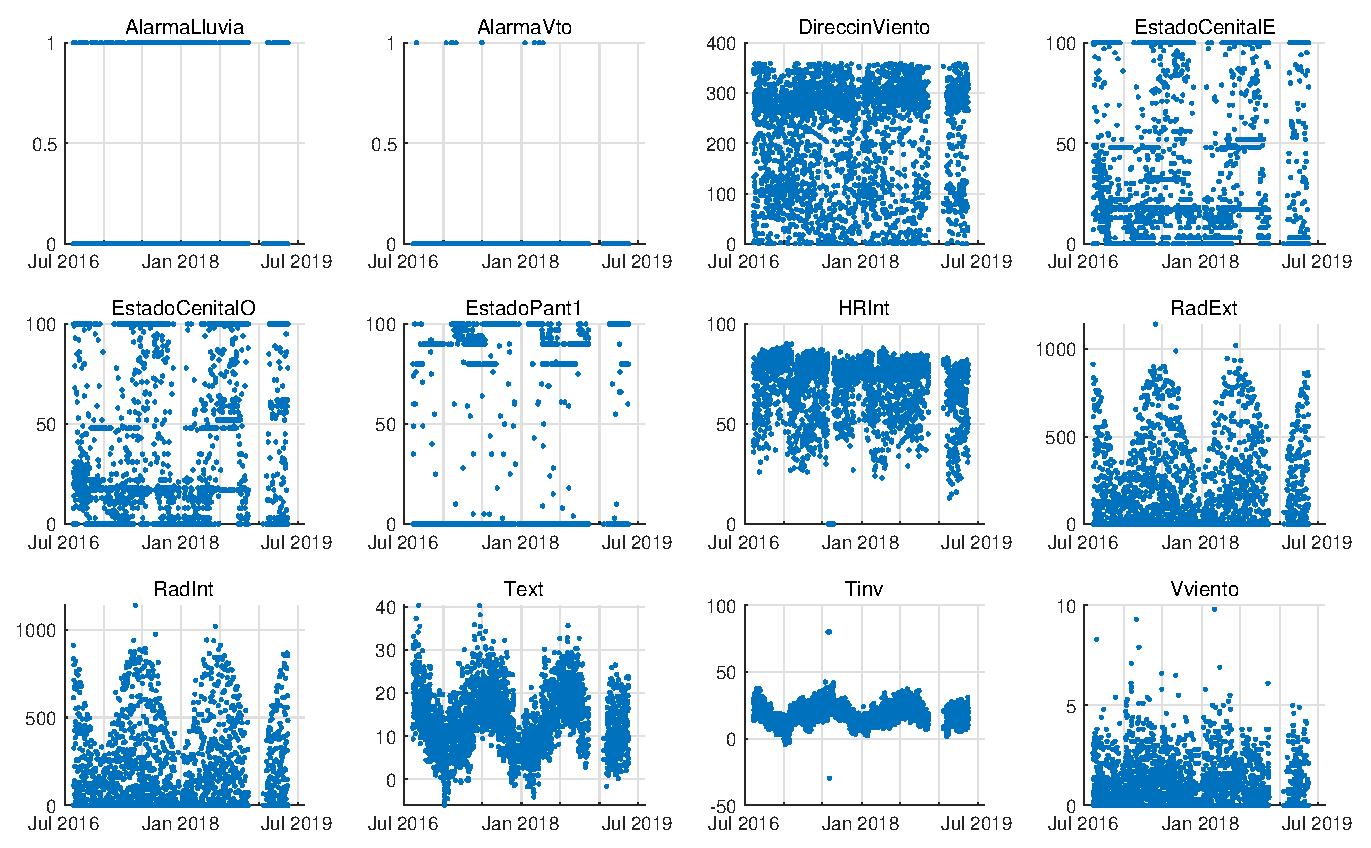
\includegraphics[scale=0.55]{img/SysClimaDataSet02.eps}
    \caption{Selection of variables}
    \label{fig:ViewDataSetSysClimaCompact}
\end{figure}

 
Las variables de la base de datos \ref{dataset:SysClimaSimply} se pueden clasificar variables dependientes e independientes. Esta clasificación separa las variables que pueden depender de otros con las variables que dependen de procesos externos. 

\begin{enumerate}
    \item Variables de Entrada
    \begin{enumerate}
        \item Perturbaciones
        \begin{enumerate}
            \item Temperatura Exterior 
            \item Radiación Exterior
            \item Velocidad del viento
            \item Dirección del viento
        \end{enumerate}
        \item Controles
        \begin{enumerate}
            \item Pantalla de Sombreo
            \item Estado de la Cenital Este
            \item Estado de la Cenital Oeste
            \item \textcolor{red}{Pellet Heater}: No tenemos este dato, pero sabemos que existe una fuente de calor adicional en el invernadero en invierno. Es conocido que este calentador funciona con un termostato a un temperatura fija de $12 ^\circ C$
        \end{enumerate}
    \end{enumerate}

    \item Variables de Salida
    \begin{enumerate}
        \item Temperatura Interior
        \item Radiación Interior
        \item Humedad Relativa Interior
    \end{enumerate}
\end{enumerate}

\section{Separación de datos con Heater}

Es conocido que una de las variables más relevantes  dentro de un invernadero es el calentador interior. Este mantiene un temperatura adecuada para la cosecha en los días de extremo frio. Concretamente en el invernadero de Meñaka se sabe que existe un calentador con un mecanismo de termostato, cuya consigna esta alrededor de $10^\circ C$. Sin embargo la señal de potencia del calentador nos ha sido capturado complicando la generación de un modelo de temperatura basado en datos. 

Es común pensar que un modelo de caja negra es capaz de simular cualquier comportamiento o función que se le ponga en frente, sin embargo para ello es necesario que la función exista. Dicho de otra manera, es necesario que el proceso a modelar solo tenga una sola una respuesta posible ante un  vector de entrada concreto, es es pues la definición de función. En el caso que nos compete, es necesario encontrar un modelo que responda de la misma manera para las misma condiciones de variables de entrada y de perturbaciones. 

El hecho de no considerar el calentador como señal de entrada hace que un modelo de caja negra intente encontrar causalidad en correlaciones no causales. Dado que conocemos que existe calentador buscaremos un procedimiento objetivo para la selección de tramos de días en los que efectivamente no existe calentador. De esta manera, la obtención de los modelos de caja negra sin tener en cuenta la señal de calentador es plausible. Luego podremos encontrar la señal de calentador con ayuda del modelo calculado previamente.

Es necesario notar que solo existen tres procesos por los que la temperatura de un cuerpo puede variar, estos son: Conducción térmica, Convección Térmica y Radiación. Dado que no tenemos modelos para estos datos es necesario utilizar el uso la conservación de energía.  

\section{Conclusion}


